\documentclass[a4paper,12pt]{article}
\usepackage{a4wide}
\usepackage{tikz}
\usetikzlibrary{calc}
\usepackage{hyperref}
\usepackage{caption}
\usepackage{enumitem}
\usepackage{amsmath}
\usepackage[font=small,labelfont=bf]{caption}

\begin{document}

\pagenumbering{arabic}
\setlist[enumerate,1]{start=0}

\setlength{\parindent}{0em}
\section*{\noindent Blockcode}
Your task is to program the behavior of an entity called ``blockcode". This entity is declared in the attached
file ``blockcode.vhdl" and has the following ports:

\begin{itemize}
	\item Input: \textit{rst} with type std\_logic; global synchronous reset
	\item Input: \textit{clk} with type std\_logic; global clock
	\item Input: \textit{data\_valid} with type std\_logic
	\item Input: \textit{data} with type std\_logic\_vector of length {{DATALENGTH}}
	\item Input: \textit{sink\_ready} with type std\_logic
	\item Output: \textit{code\_valid} with type std\_logic
	\item Output: \textit{code} with type std\_logic\_vector of length {{CODELENGTH}}

\end{itemize}

\begin{center}
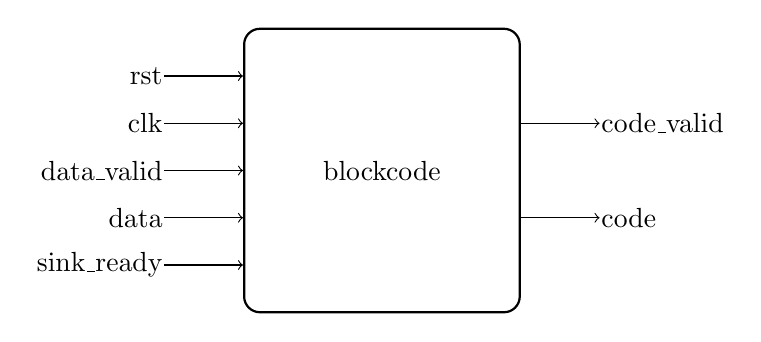
\begin{tikzpicture}
\draw node [draw,rectangle, minimum height=36mm, minimum width=35mm,rounded corners=2mm,thick](entity){};

\draw[->] ($ (entity.west)+(-10mm,12.0mm)$) -- ($ (entity.west) + (0mm,12.0mm)$);
\draw[anchor=east] node at ($ (entity.west)+(-9mm,12.0mm)$){ rst };

\draw[->] ($ (entity.west)+(-10mm,6.0mm)$) -- ($ (entity.west) + (0mm,6.0mm)$);
\draw[anchor=east] node at ($ (entity.west)+(-9mm,6.0mm)$){ clk };

\draw[->] ($ (entity.west)+(-10mm,0.0mm)$) -- ($ (entity.west) + (0mm,0.0mm)$);
\draw[anchor=east] node at ($ (entity.west)+(-9mm,0.0mm)$){ data\_valid };

\draw[->] ($ (entity.west)+(-10mm,-6.0mm)$) -- ($ (entity.west) + (0mm,-6.0mm)$);
\draw[anchor=east] node at ($ (entity.west)+(-9mm,-6.0mm)$){ data };

\draw[->] ($ (entity.west)+(-10mm,-12.0mm)$) -- ($ (entity.west) + (0mm,-12.0mm)$);
\draw[anchor=east] node at ($ (entity.west)+(-9mm,-12.0mm)$){ sink\_ready };


\draw[->] ($ (entity.east) + (0mm,6.0mm)$) -- ($ (entity.east) + (10mm,6.0mm)$);
\draw[anchor=west] node at ($ (entity.east) + (9mm,6.0mm)$){ code\_valid };

\draw[->] ($ (entity.east) + (0mm,-6.0mm)$) -- ($ (entity.east) + (10mm,-6.0mm)$);
\draw[anchor=west] node at ($ (entity.east) + (9mm,-6.0mm)$){ code };


\draw node at ($ (entity) - (0,0mm)$){ blockcode };

\end{tikzpicture}
\end{center}

Do not change the file ``blockcode.vhdl".\\

This entity should work as an intermediate unit, that creates blockcode elements from given data elements and transmits
them to the following data sink as seen in Figure 1. In the following sections the transmission and the encoding will
be discussed in depth.
\\

\begin{figure}[h!]
\centering
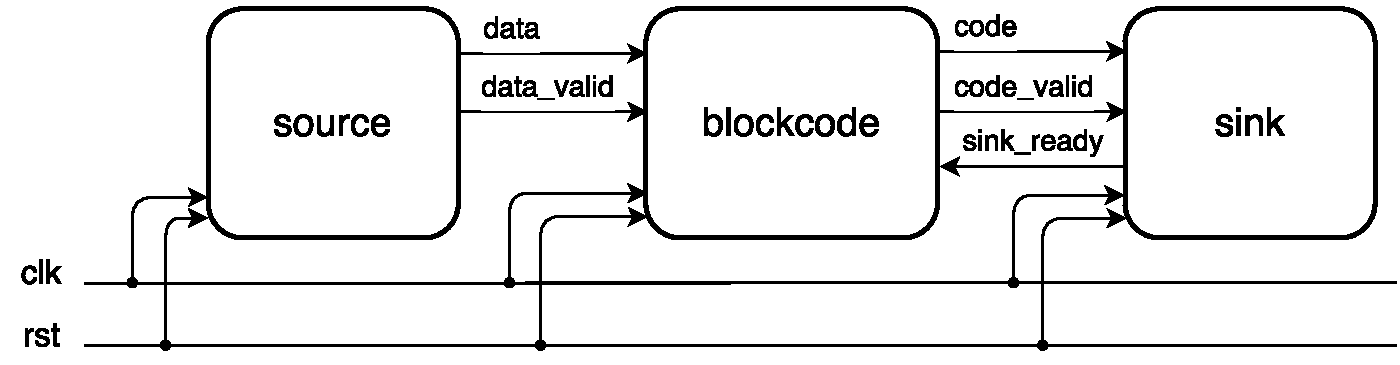
\includegraphics[scale=0.6]{../static/system_view.pdf}
\caption{System view. The source creates data to be encoded by your entity, which sends the blockcode encoded data to
the following data sink.}
\end{figure}

\newpage
\subsection*{\noindent Transmission}

\textbf{Transmission data source $\rightarrow$ ``blockcode" entity:} This transmission is with the following ports:
\begin{itemize}
\item \textbf{data:} contains the data which is to be encoded as blockcode.
\item \textbf{valid\_data:} indicates if the data on the port \textit{data} is valid in the clock cycle.
The ``blockcode" entity should only encode valid data.
\end{itemize}

\textbf{Transmission ``blockcode" entity $\rightarrow$ data sink:} This is a connection with sink backpressure,
meaning the sink can indicate if it is ready to receive data. It takes place with the following ports:
\begin{itemize}
\item \textbf{code:} contains the code which was generated by encoding given valid data on the port \textit{data}.
\item \textbf{code\_valid:} indicates if the code at the port \textit{code} is valid in the clock cycle.
\item \textbf{sink\_ready:} indicates if the sink is ready to receive code.
\end{itemize}

\textbf{Backpressure:} If the sink is not ready to receive it unsets the port \textit{sink\_ready} (\textit{sink\_ready} = 0).
The ``blockcode" entity sends the same code until the sink it is ready. The sink only captures code if both
\textit{code\_valid} and \textit{sink\_ready} are set.\\
\\
\textbf{Buffering:} As the sink can stall the transmission you will need a buffer in the ``blockcode" entity (e.g. circular FIFO).
Your buffer needs to be able to buffer a maximum of 3 elements for this task. \\
\\
\textbf{Synchronous outputs:} All outputs of entities in the system are registered to the common clock \textit{clk},
meaning that changes on these ports only happen at the rising edge of the common clock \textit{clk}.\\

\newpage
\subsection*{\noindent Encoding}

The dataword has to be encoded as a $[{{CODELENGTH}},{{DATALENGTH}}]$ blockcode, meaning
{{DATALENGTH}} data bits are padded with {{NUMPARITY}} parity bits:

\begin{equation}
d = (d_0,d_1, .. d_{{LASTDATAELEM}}) \longrightarrow c = (d_0,d_1,...,d_{{LASTDATAELEM}},p_0,...,p_{{LASTPARITYELEM}})
\end{equation}

The encoding is done with the help of a generator matrix G:

\begin{equation}
c = d \cdot G
\end{equation}

Use the given generator matrix consisting of an identity matrix and the parity matrix (separated by a vertical line):

\begin{center}
\[
\left(
\begin{array}{ {{MATRIXHEADER}} }
{{GENERATORMATRIX}}
\end{array}
\right)
\]
\end{center}

\textbf{Tip:} As + in binary is the same as XOR, use XOR to calculate the parity. \\
\\

\textbf{Encoding example:} ({{EXAMPLEDATA}}) $\longrightarrow$ ({{EXAMPLECODE}}) \\

\newpage
\subsection*{\noindent System behavior}

\begin{figure}[h!]
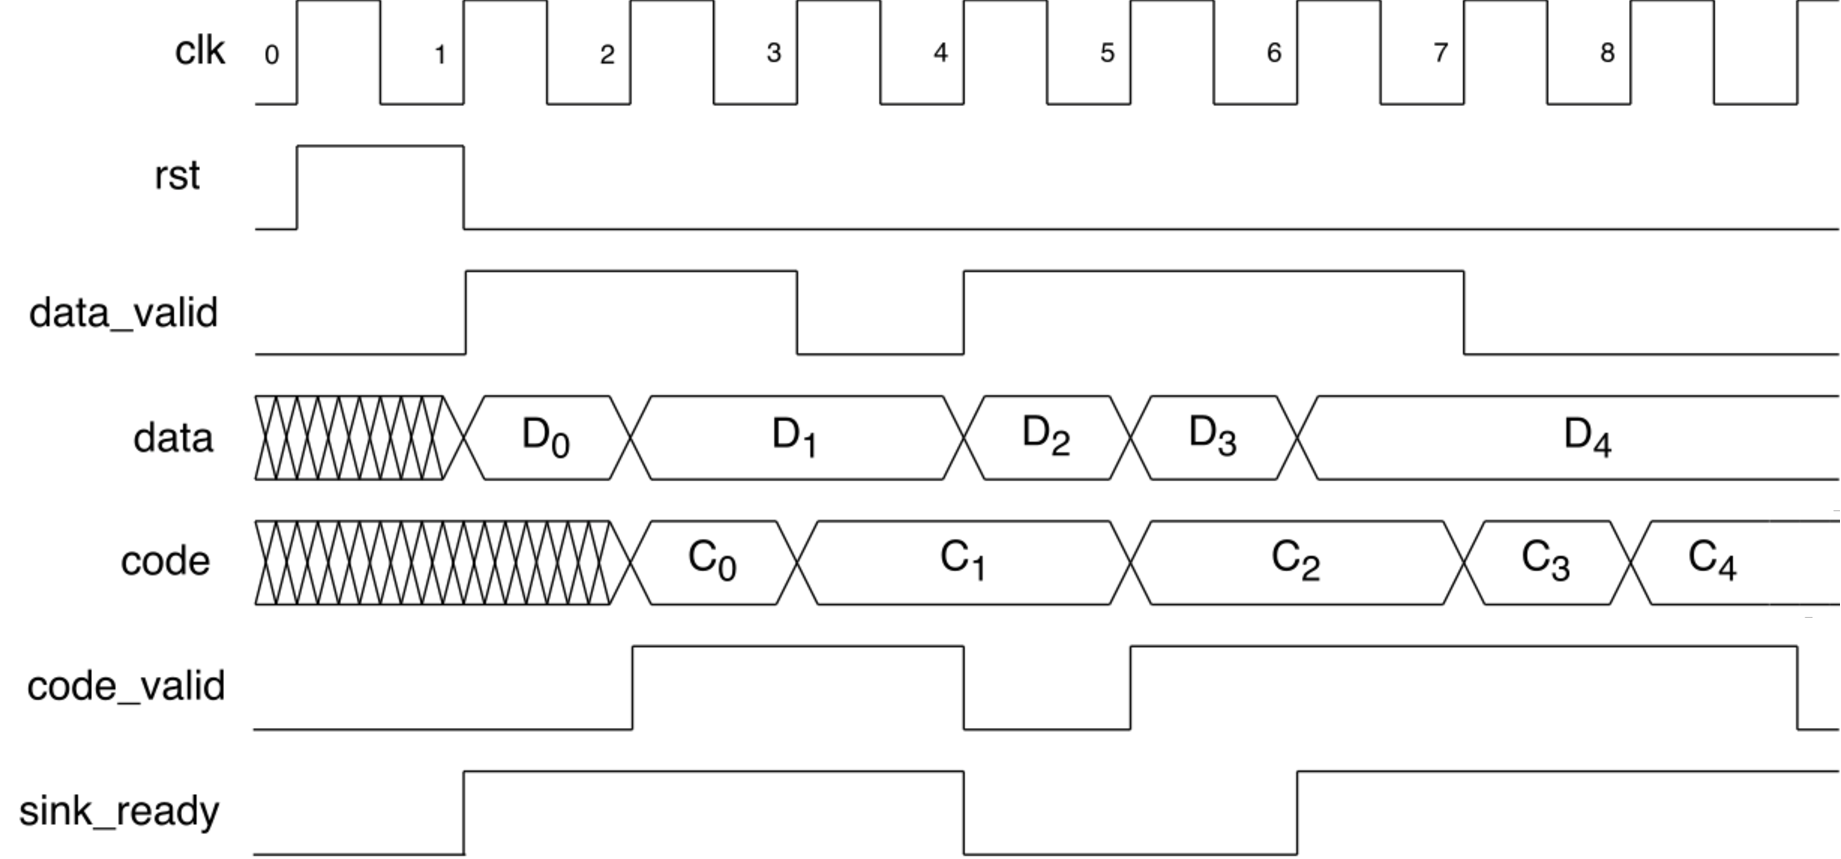
\includegraphics[scale=0.5]{../static/diagram.pdf}

\caption{Example behavior of the whole system. The numbers denote the start of clock cycles.}
\end{figure}

Figure 2 illustrates the desired behavior of the entity ``blockcode" by example for each clock cycle:
\begin{enumerate}
\item Global reset.
\item A valid data element $D_0$ is given. This is indicated by a \textit{data\_valid} being set.
\item A new valid data element $D_1$ is given. The encoded element $C_0$ is set to be transmitted. The sink is ready as seen by the set \textit{sink\_ready}. Therefore the sink captures the code element in this clock cycle.
\item No new valid data element is given, as seen by the unset \textit{data\_valid}. The encoded element $C_1$ is set to be transmitted and captured by the sink.
\item A new valid data element $D_2$ is given. As $C_1$ was already captured, the set code element is not valid, no transmission will occur. Therefore \textit{code\_valid} is unset.
\item A new valid data element $D_3$ is given. The encoded element $C_2$ is set to be transmitted and captured by the sink. The sink is not ready to capture as seen by the unset \textit{sink\_ready}.
\item A new valid data element $D_4$ is given. As $C_2$ was not captured in the last cycle it remains set. The sink is ready again and captures $C_2$.
\item No new valid data element is given. $C_3$ is set and captured.
\item No new valid data element is given. $C_4$ is set and captured.
\end{enumerate}

\newpage

The described  behavior has to be programmed in the attached file ``blockcode\_beh.vhdl".\\

To turn in your solution write an email to {{SUBMISSIONEMAIL}} with Subject ``Result Task {{TASKNR}}" and attach your behavior file(s):
\begin{itemize}
\item ``blockcode\_beh.vhdl"
\end{itemize}

\vspace{0.7cm}
Good Luck and May the Force be with you.


\end{document}
